\documentclass[11pt,a4paper,titlepage]{article}

%\usepackage{pdflscape}
\usepackage[margin=1in]{geometry}
\usepackage{titling}
\usepackage{graphicx}
\usepackage[hidelinks]{hyperref}
\usepackage{float}
\usepackage{titlesec}

\setcounter{secnumdepth}{4}

\DeclareGraphicsExtensions{.png}
\graphicspath{ {img/} }


\newcommand{\subtitle}[1]{%
  \posttitle{%
    \par\end{center}
    \begin{center}\large#1\end{center}
    \vskip0.5em}%
}

\titleformat{\paragraph}
{\normalfont\normalsize\bfseries}{\theparagraph}{1em}{}
\titlespacing*{\paragraph}
{0pt}{3.25ex plus 1ex minus .2ex}{1.5ex plus .2ex}


\begin{document}
\title{Crowd Source User Manual}
\subtitle{ Git: \url{https://github.com/FrikkieSnyman/COS301_GroupProject}\\
Client: Epi-Use
}

\author{\textbf{COS301 Main Project - The fellowship of the CIN}\\
Frikkie Snyman 13028741\\
Hanrich Potgieter 12287343\\
Hugo Greyvenstein 13019989\\
Andre Calitz 13020006\\
Chris Cloete 13029721\\}

\maketitle1

\tableofcontents
\pagebreak

\setlength{\parindent}{0em}
\setlength{\parskip}{0.5em}
\section{System Overview}
	This system is designed to assist on estimations for various tasks, by providing an interface for designing project trees, performing estimations on those trees, and generating conclusive reports based on those estimations.

Estimations refer to quantities that are assigned to descriptive tasks, based on the time it is estimated to take to build that task. This methodology typically forms part of any Agile Software Development process.

Project owners can create new project trees, which consist of various tasks and sub-tasks. Any registered user can be a project creator, and therefore the owner of said project. With the creation of a new project, the owner is prompted to add users that has the right to estimate on that specific project. These users are refered to as Estimators for the project.

Estimators are notified of newly created projects on which they may estimate. After estimation is done, which is the event where all Estimators have completed estimation, the Owner is notified, and reports are generated for these estimations. Based on these reports, the Owner can prompt to reopen estimation, and discuss previous estimations.
\section{System Configuration}
	The system is intended to run on the cloud, where it will act as a host for a web page. This web page can then be accessed by any browser. Seeing as the system is responsive, any window size can be used for access.

A mobile application can also be used to gain access to the services provided.
\section{Installation}
	\begin{figure}[H]
	    	\centering
	    	\fbox{
\includegraphics[width=0.5\textwidth]{MEAN}}
	    	\caption{MEAN.js logo}
	    	\label{fig:MEAN}
   	\end{figure}
The installation is quite an easy process as estimate swarm uses standard web technologies. We can deploy our system in one of two ways. One way is to use a docker image to load the system the other is to set it up by loading all the dependancies to a machine. Estimation swarm is using the mean stack so should you encounter any issues please consult their webpage. \url{http://mean.io}. The github readme also houses the installation instructions.
\subsection{Setting up the environment}
To use our application the following prerequisites need to be met. Please note that installing packages globally requires super user privillages on unix based systems and administrator privileges on windows.
\begin{itemize}
	\item git. It is important to have a good understanding of this technology. It must be installed on your system for development.
	\item NPM(Node Package manager) and node.js
	For the latest information on installing npm please visit \url{https://nodejs.org/download/} Once you have this setup properly it is important to make sure you have the latest version installed.
	\item BOWER for client side dependancies.
	This technologie works with our stack and the latest version can be installed by making use of npm.
	\newline
	npm install -g bower
	\item MongoDB document database. Mongo has different installation instructions based on the operating system being used thus it is best to consult the following website \url{https://www.mongodb.org} for the instructions.
	\item GRUNT task manager. GRUNT can be installed through npm. 
	\newline
	npm install -g grunt-cli
\end{itemize}
Estimation swarm is now ready to be started. First make sure that Mongodb is up and running. Next clone the project form gitHub by running the following command.
\newline
git clone \url{https://github.com/FrikkieSnyman/COS301_GroupProject.git}
\newline
Install the dependancies by running the following command.
\newline
npm install
\newline
Running the grunt command in the root directory of the project will start the server. The server will start in the development environment on port 3000 by default. Estimation swarm currently supports running in three environment types.
\begin{itemize}
	\item{Development} is used to run the server for development, non minified files are used so that errors can be properly shown.
	\item{Production} loads all the minified sources and also only non development dependancies. This is the method to use when running the server for commercial use.
	\item{Secure} is just a enhanced version of production with added ssl security. For this environment to work it requires the necessary certificates.
\end{itemize}
After this the server should be functioning and you can move on to getting started. Check your favourite web browser and the server should be running on port 3000.
\subsection{Using docker}
This is still under development and will be implemented soon.
\url{http://docs.docker.com/mac/started/}
\subsection{Deploying on your server}
Changing environment setting to suite your current need is quite easy. Under your project directory there is a config folder. It contains all the variable that can be changed for the various services. Using passport.js for authentication allows you to integrate with the various services for authentication. We currently support Facebook, Google and Twitter authentication. Please visit \url{http://passportjs.org} for further instructions on how to configure this services. We recommend using digital ocean servers to run this project on. \url{https://www.digitalocean.com}

\subsection{Installation failures}
Should the installation fail please make sure that all the MEAN.js dependancies are installed by visiting their website. If the issue cannot be resolved please log a issue on gitHub.
\section{Getting Started}
	\subsection{Getting on to the System}
\begin{itemize}
	\item{Sign up your account}
	\newline
	You will need to add an account to be able to sign into the system.
	\begin{figure}[H]
	    	\centering
	    	\fbox{\includegraphics[width=0.5\textwidth]{SignUP}}
	    	\caption{Sign Up}
	    	\label{fig:Learning rate 0.1}
   	\end{figure}
	\item{Sign in}
	\newline
	After your account has been created, you will have to sign in.
	\begin{figure}[H]
	    	\centering
	    	\fbox{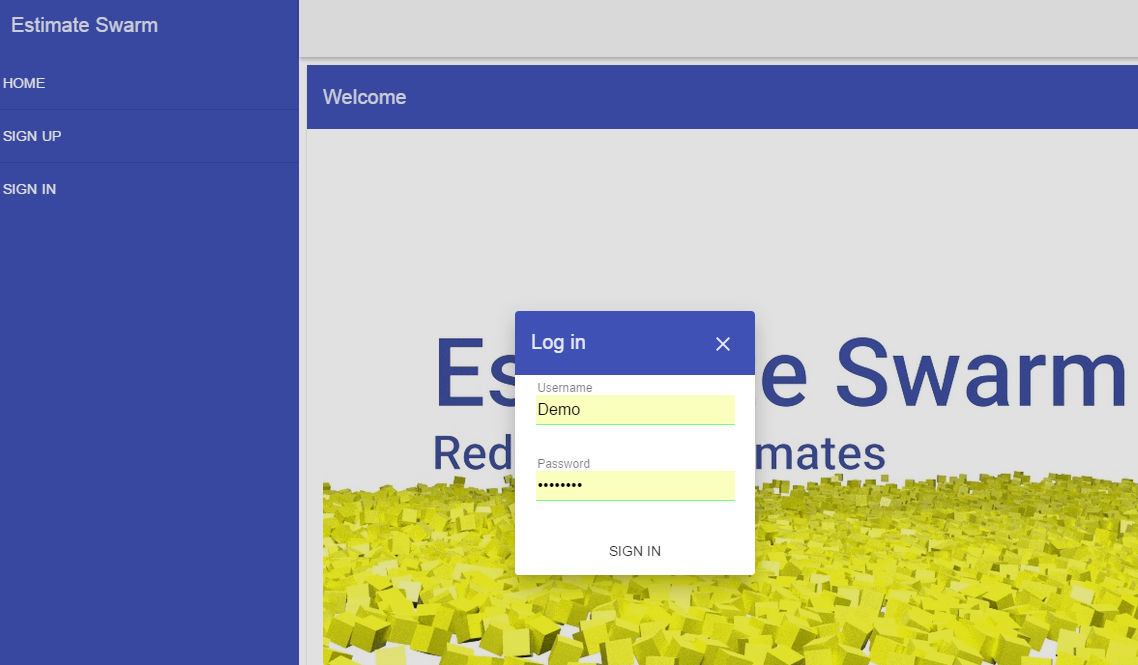
\includegraphics[width=0.5\textwidth]{login}}
	    	\caption{Login}
	    	\label{fig:Learning rate 0.1}
   	\end{figure}
\end{itemize}
\subsection{My Profile}
\begin{itemize}
	\item{Edit Profile Details}
	\newline
	After you account has been created and you are signed in, you can access your information on the "Profile" page. You can navigate there from another other page, while signed in, by clicking on the "Profile" tab in the left hand side navigation. Here you can edit your account information as shown in the figure below. After you are done editing, you can save your changes by clicking the "Save Profile" button at the bottom of the screen.
	\begin{figure}[H]
	    	\centering
	    	\fbox{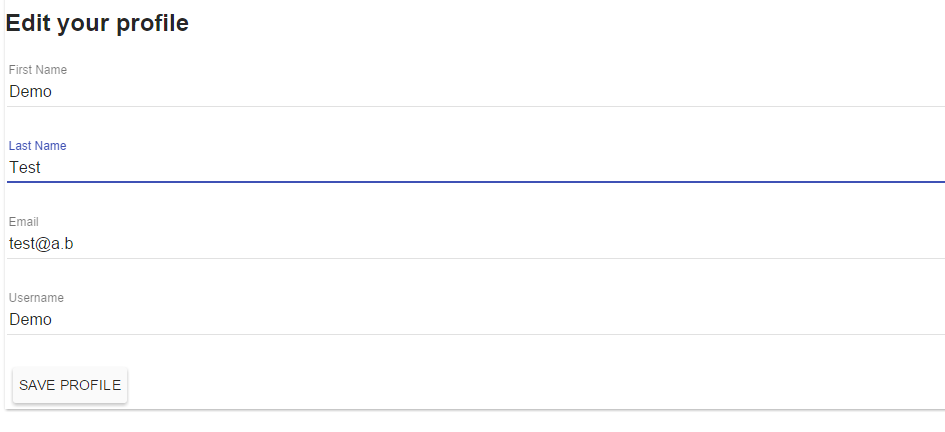
\includegraphics[width=0.5\textwidth]{profile}}
	    	\caption{Profile Page}
	    	\label{fig:Learning rate 0.1}
   	\end{figure}
\end{itemize}
\section{Using the system}
	\subsection{Creating a project}
\begin{itemize}
	\item{Navigate to projects list page}
	\newline
	After you have signed in you will be navigated to the projects list page, if you wish to navigating there from another page, you can simply click on the projects tab on the left side navigation bar.
	\begin{figure}[H]
	    	\centering
	    	\fbox{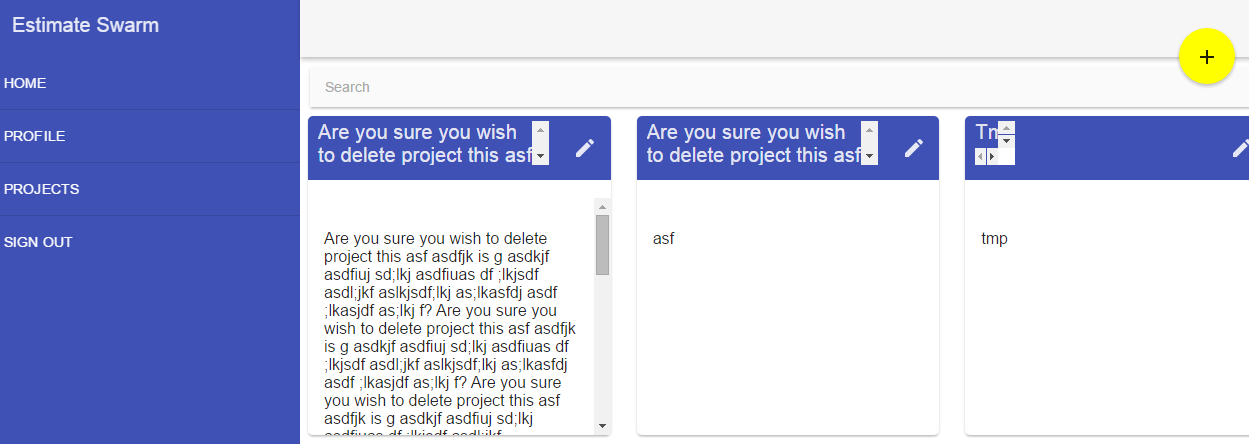
\includegraphics[width=0.5\textwidth]{projectsList}}
	    	\caption{Projects List Page}
	    	\label{fig:Learning rate 0.1}
   	\end{figure}
	\item{Add a new project}
	\newline
	On the projects list page, you can simply click on the "add project" button that is in the top right hand corner of the screen.
	\begin{figure}[H]
	    	\centering
	    	\fbox{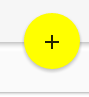
\includegraphics[width=0.5\textwidth]{addButton}}
	    	\caption{Add Project Button}
	    	\label{fig:Learning rate 0.1}
   	\end{figure}
	\item{Complete details of the project}
	\newline
	On the "Create Project" page you will have to fill in the details of the project in order to complete the creation of the project. You will have to give the project a name and a description. You will also have to indicate who will be allowed to estimate on the project as shown in the figure below.
	\begin{figure}[H]
	    	\centering
	    	\fbox{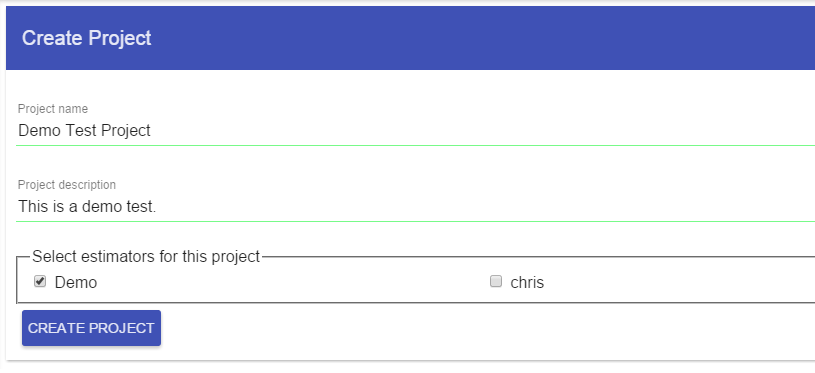
\includegraphics[width=0.5\textwidth]{createProj}}
	    	\caption{Create Project Page}
	    	\label{fig:Learning rate 0.1}
   	\end{figure}
\end{itemize}
\subsection{Estimation Process}
\begin{itemize}
	\item{Create Project Tree}
	\newline
	From here you will have to create a project tree that represents the project that you need an estimation on. You can do this by adding nodes, this is done by clicking on the "Add node" button, to the project tree and naming them appropriately. You can save the tree by clicking on the "Save Project" button to continue editing the tree at a later point. When you are satisfied with the tree, you can open it for estimation, by clicking on the "Open For Estimation" button. After the project has been opened for estimation, it can not be edited again. Emails will be sent out the users that were chosen to estimate on the project to inform them that the project is now available for estimation.
	\begin{figure}[H]
	    	\centering
	    	\fbox{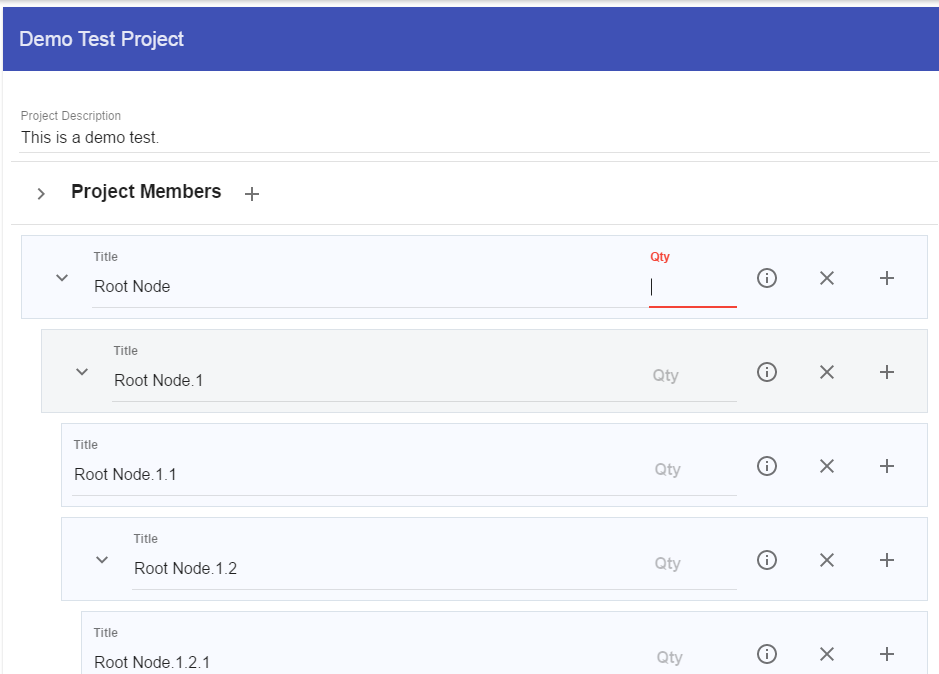
\includegraphics[width=0.5\textwidth]{createTree}}
	    	\caption{Create Tree Page}
	    	\label{fig:Learning rate 0.1}
   	\end{figure}
	\item{Estimating}
	\newline
	The estimators can now estimate on each of the leaf nodes of the project. The values on the leaf nodes will then bubble up to their parent nodes, all the way up the tree to the root node. This value at the highest root node, then gives the total value of the whole tree, i.e. the total estimation that the estimator estimated on the project. When the estimator is done, he/she can click on the "Submit Estimation" button to submit his/her estimation to the project owner.
	\begin{figure}[H]
	    	\centering
	    	\fbox{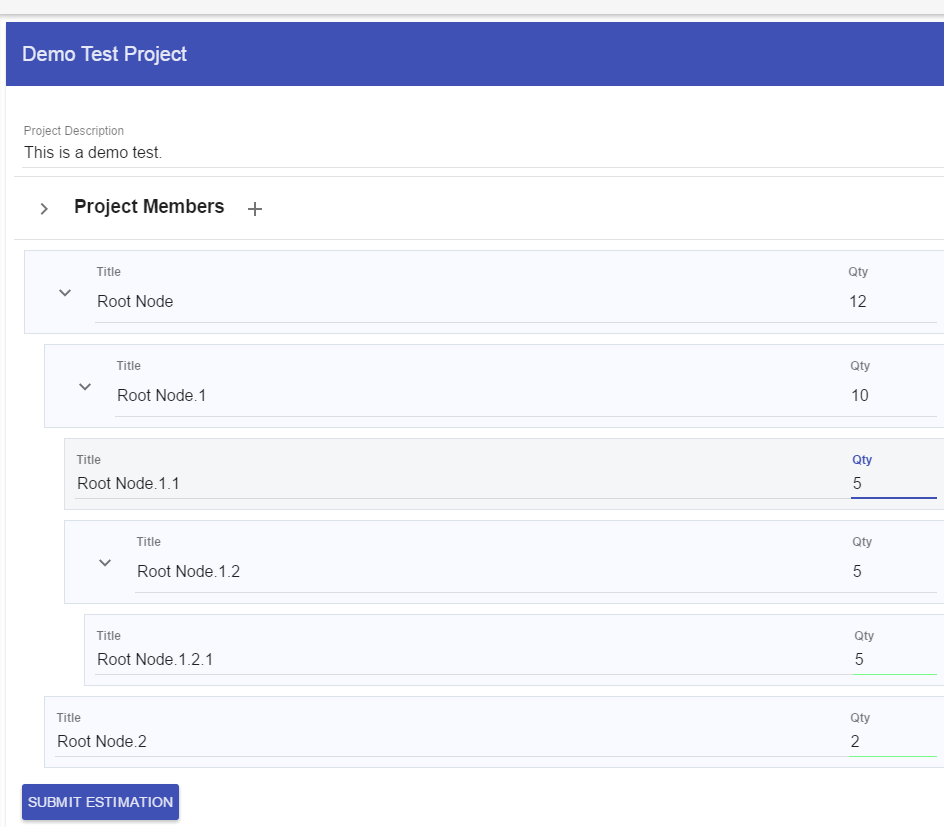
\includegraphics[width=0.5\textwidth]{estimate}}
	    	\caption{Estimation Page}
	    	\label{fig:Learning rate 0.1}
   	\end{figure}
\end{itemize}
\subsection{Reporting}
\begin{itemize}
   	\item{Report list}
	\newline
	After all estimations have been done by the different estimators, a report is created. It can then be accessed via the "Reports" tab in the side navigation bar.
	\begin{figure}[H]
	    	\centering
	    	\fbox{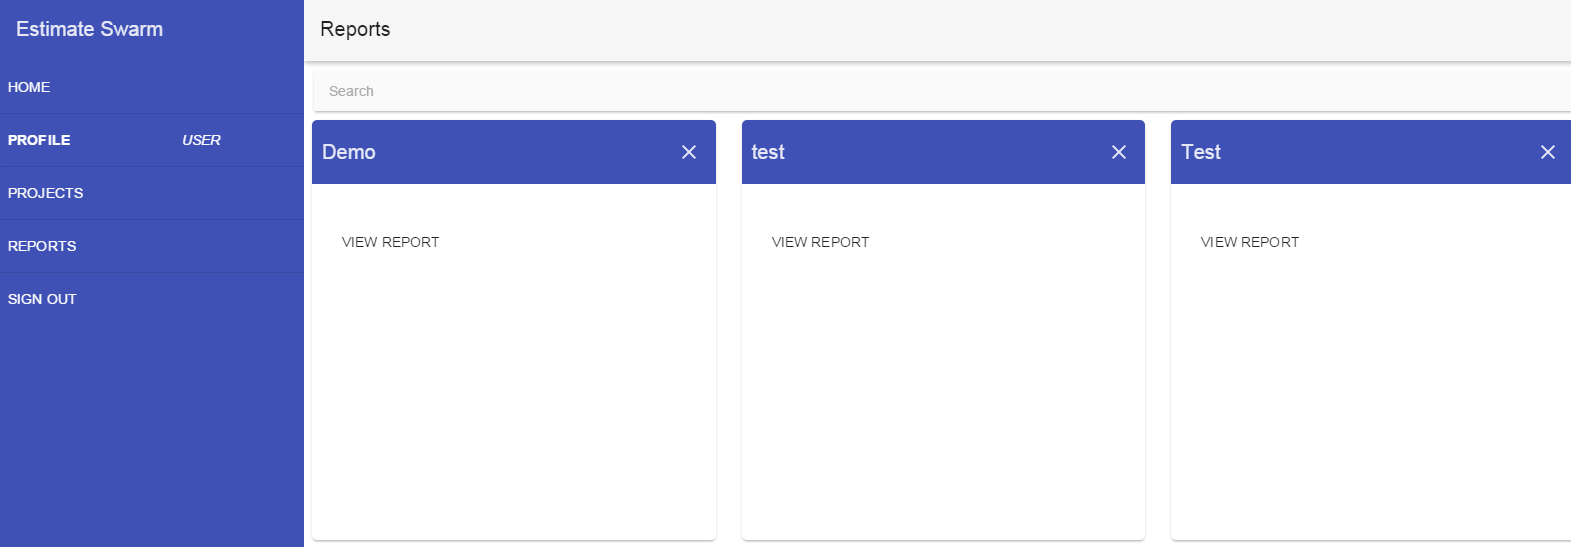
\includegraphics[width=0.5\textwidth]{reportlist}}
	    	\caption{Reports Page}
	    	\label{fig:Learning rate 0.1}
   	\end{figure}
   	\pagebreak
   	\item{Report of Project}
	\newline
	The report system consists of two graphic reports which are a bar graph and a box plot to show the relationships of the estimations of the different modules in the tree projects.
	\begin{figure}[H]
	    	\centering
	    	\fbox{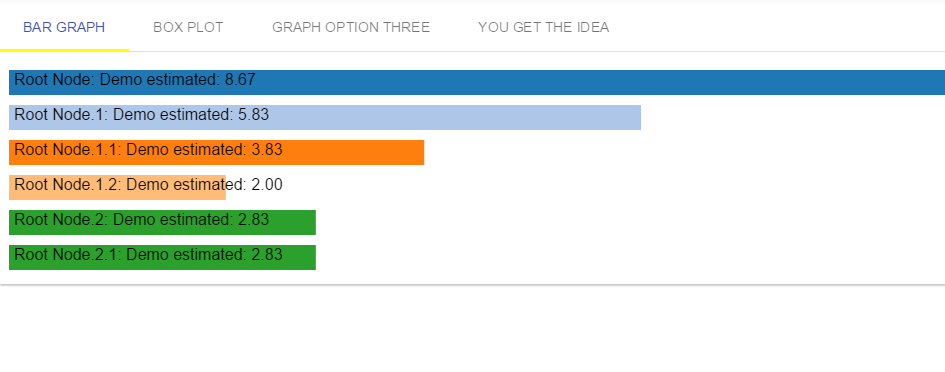
\includegraphics[width=0.5\textwidth]{bar}}
	    	\caption{Bar Graph}
	    	\label{fig:Learning rate 0.1}
   	\end{figure}
   	\begin{figure}[H]
   			\centering
	    	\fbox{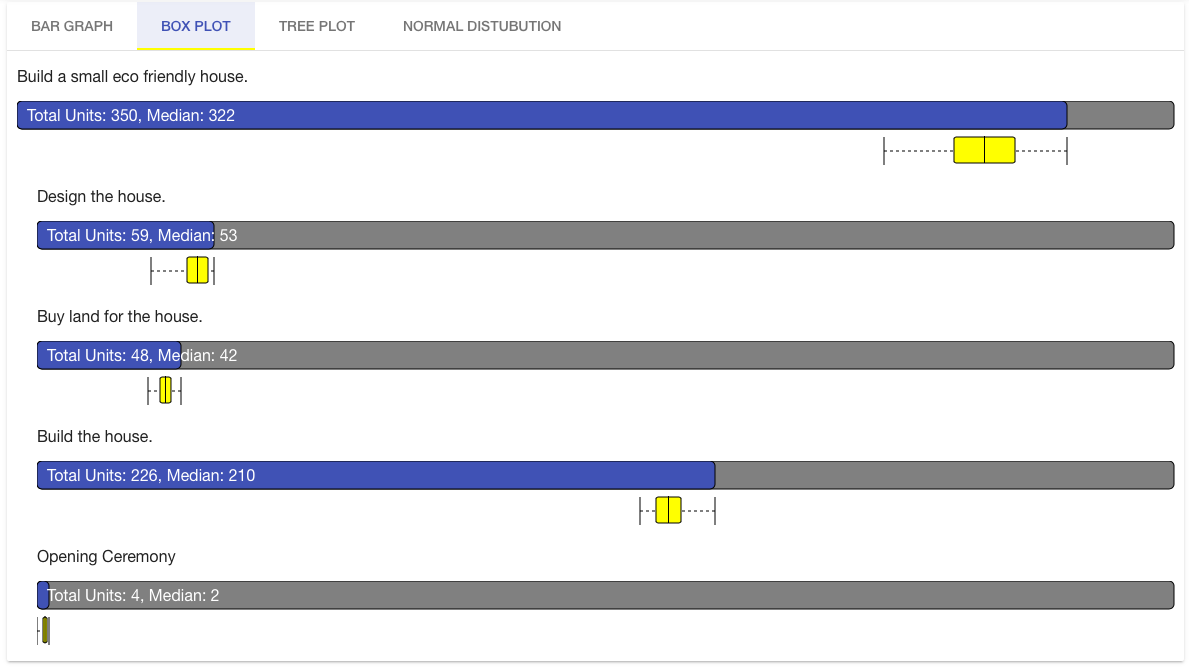
\includegraphics[width=0.5\textwidth]{boxplot}}
	    	\caption{Box Plot}
	    	\label{fig:Learning rate 0.1}
   	\end{figure}
\end{itemize}
\pagebreak
\section{Troubleshooting}
	While working on a project tree, the user must explicitly save the project tree for changes to be persisted to the database. This can be done by clicking on the "Save Project" button, as seen in the bottom left corner of the figure below

	\begin{figure}[H]
	    	\centering
	    	\fbox{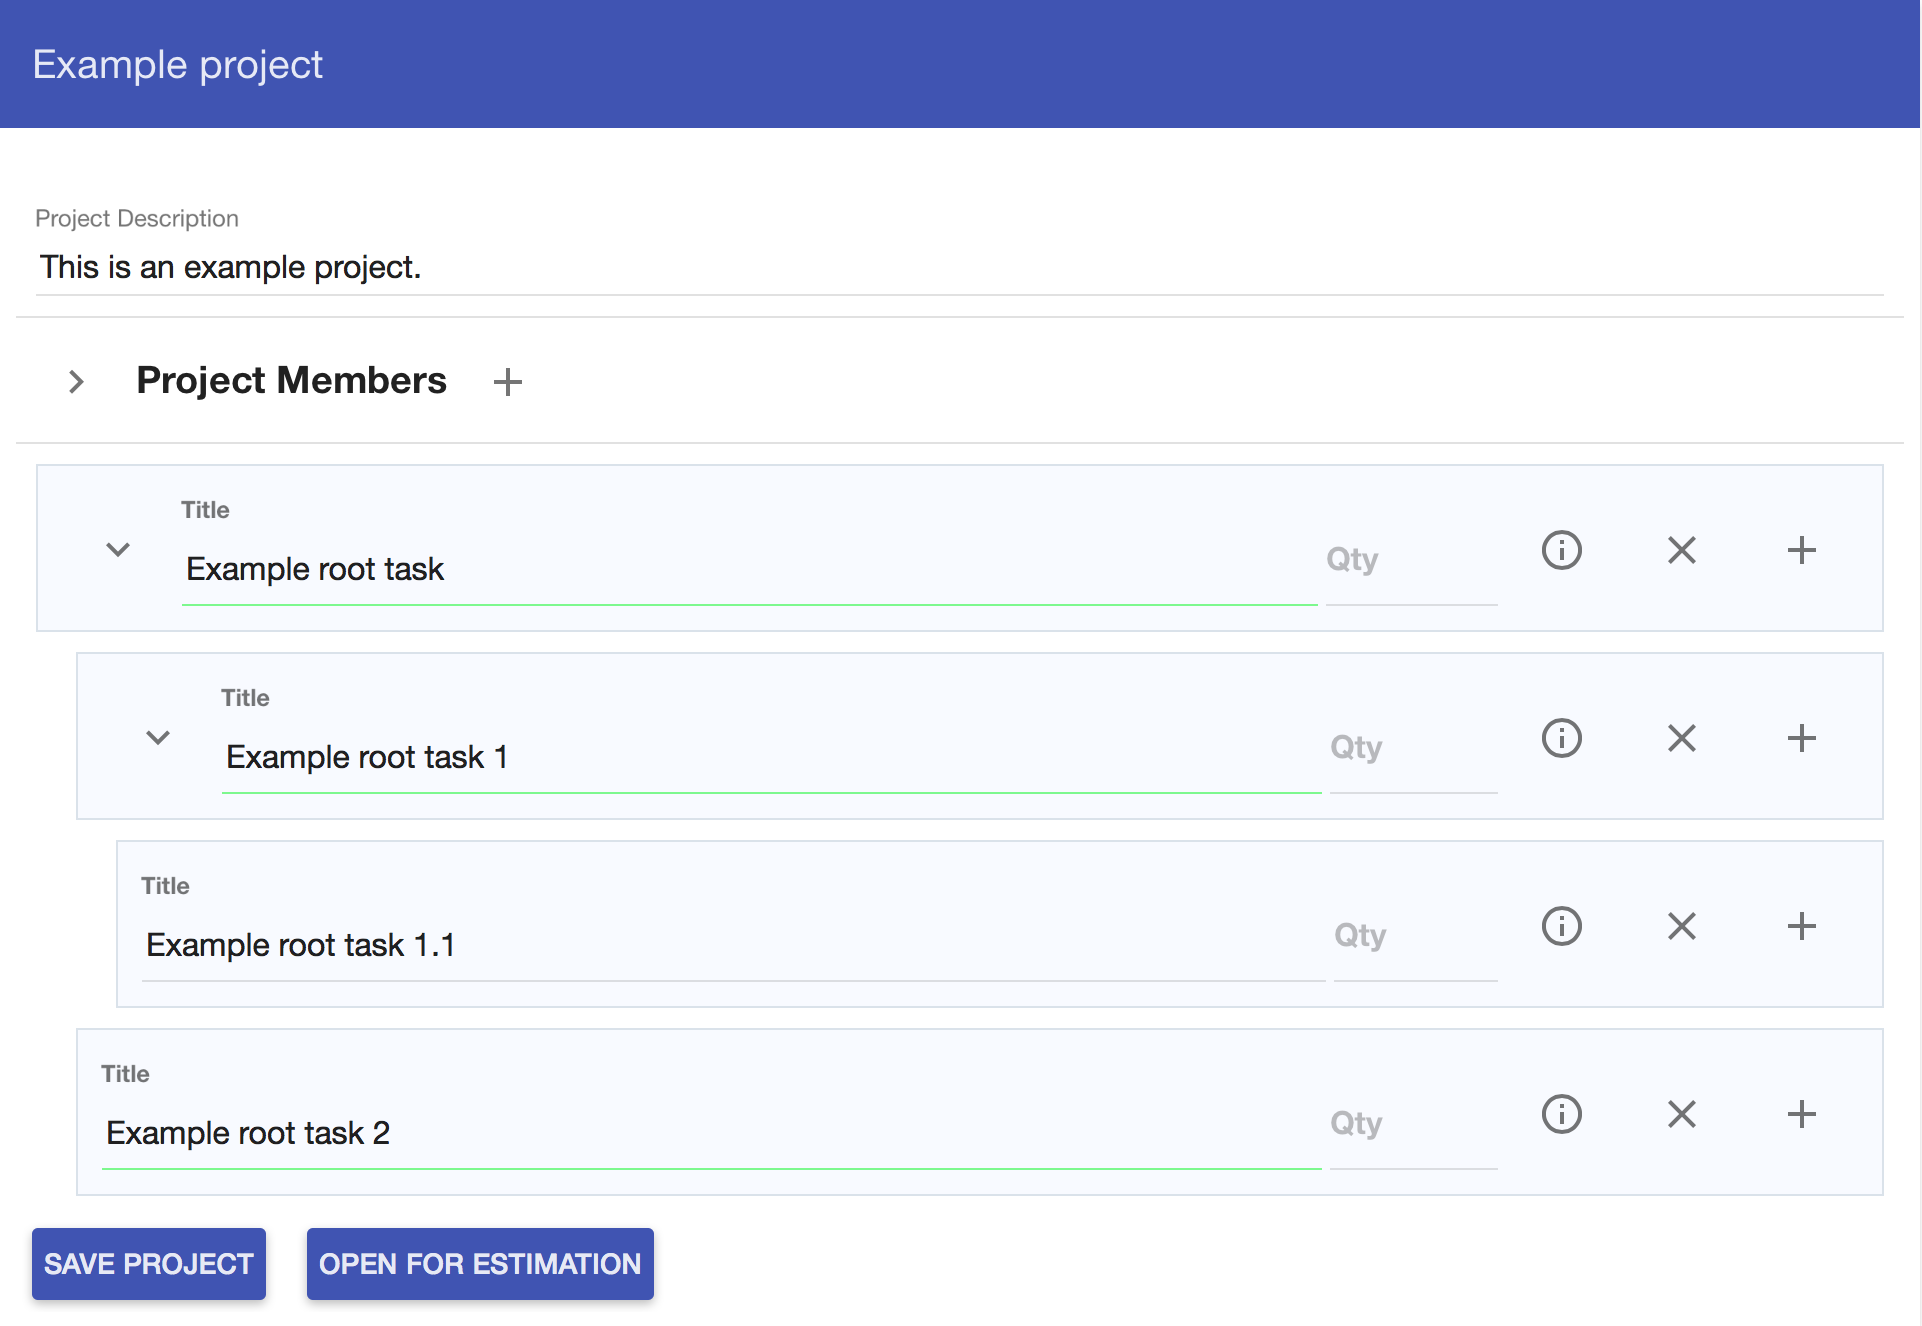
\includegraphics[width=0.5\textwidth]{saveProject}}
	    	\caption{Save Project}
	    	\label{fig: Save Project}
   	\end{figure}

If the user has not saved the project tree, and attempts to navigate away from the edit project page, the user will be prompted with the confirmation dialog displayed in the figure below.

	\begin{figure}[H]
	    	\centering
	    	\fbox{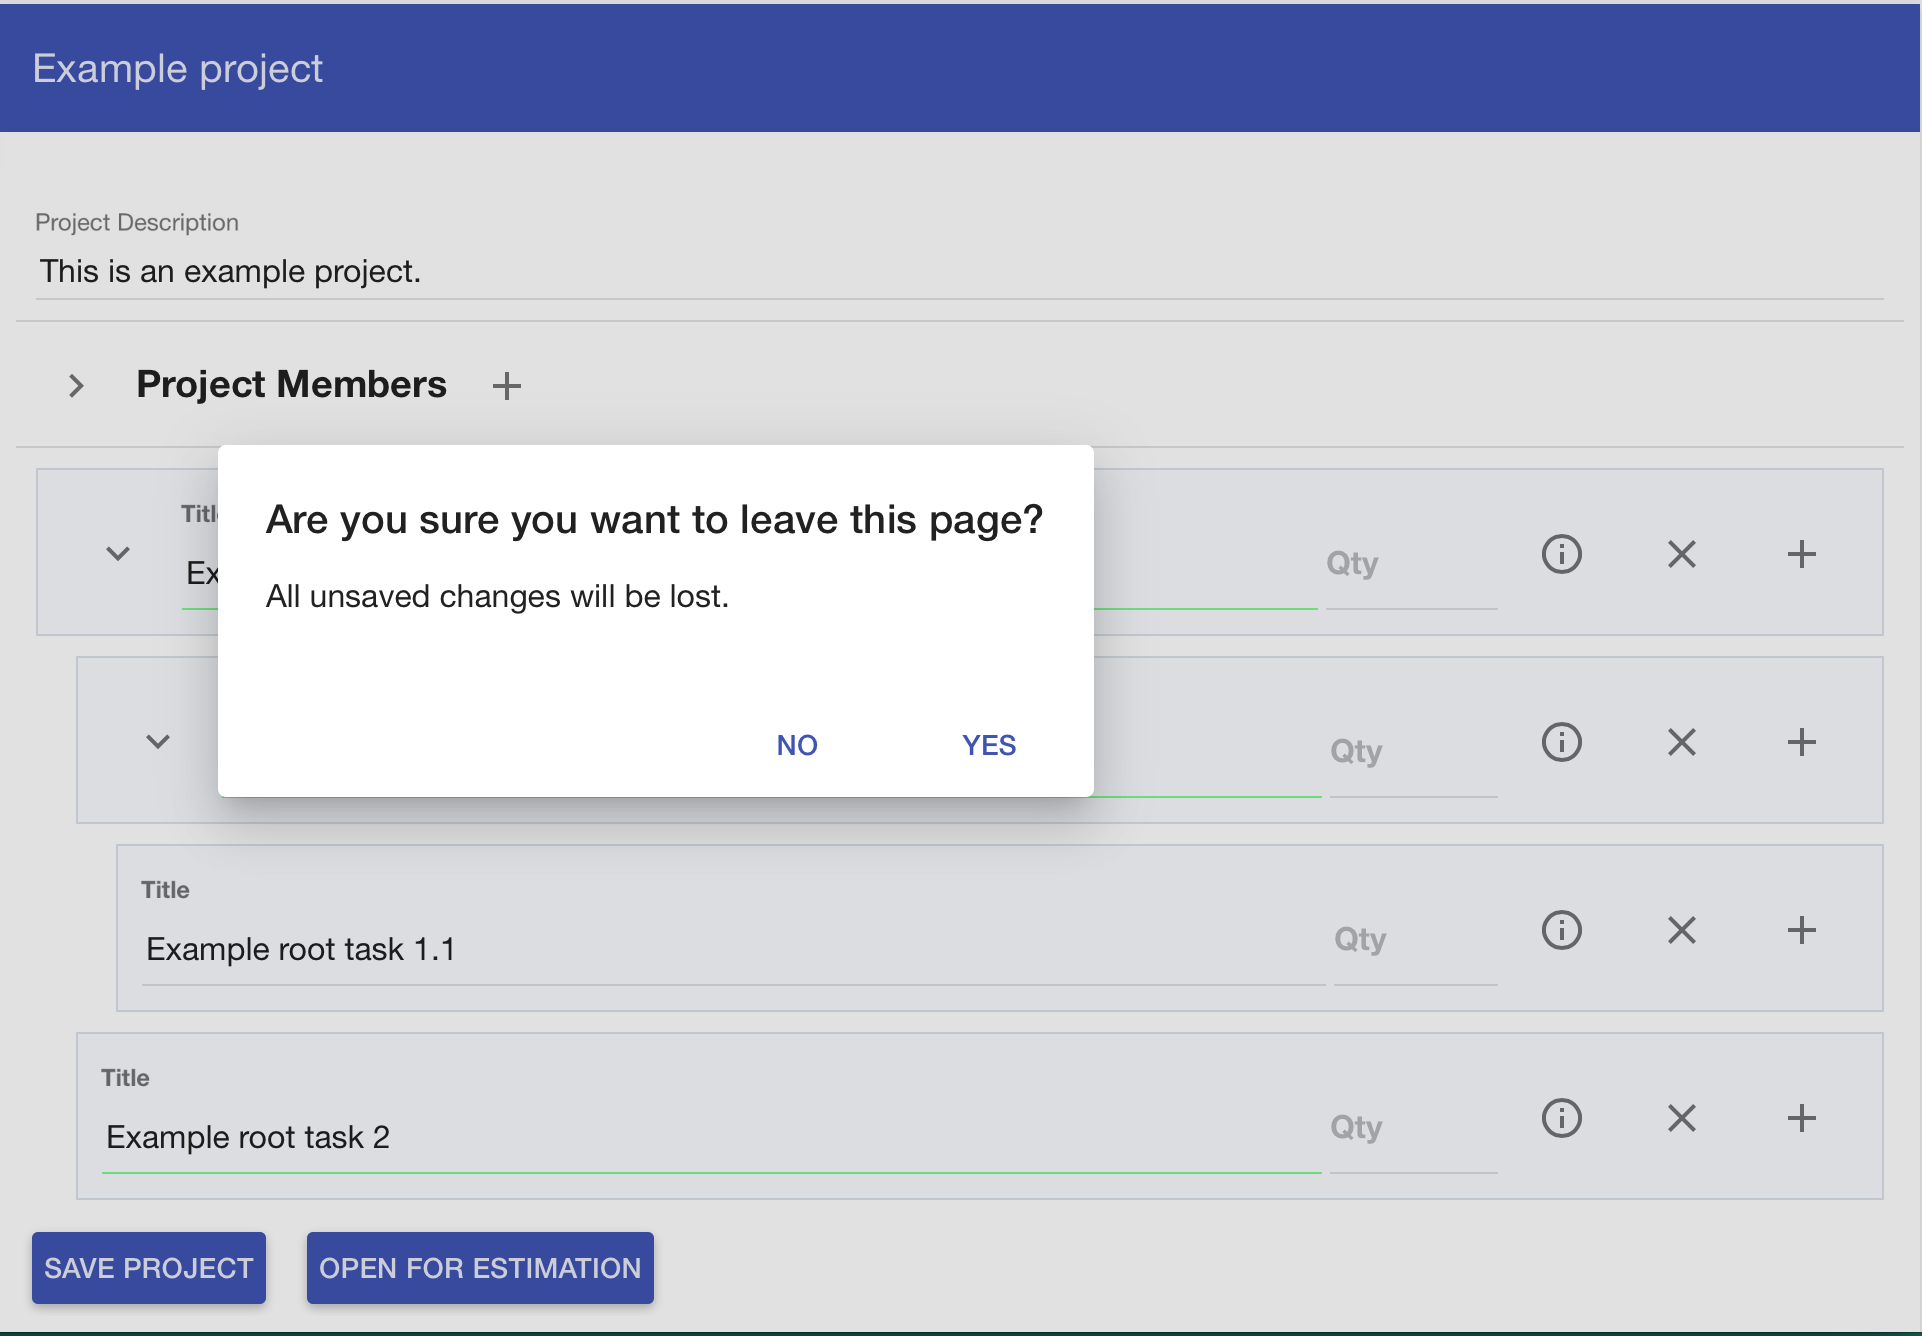
\includegraphics[width=0.5\textwidth]{confirmNavigateAway}}
	    	\caption{Confirmation of navigation away}
	    	\label{fig: Confirmation}
   	\end{figure}

If the user wishes to discard changes, he/she can navigate away from the page without saving the changes. Otherwise, the user can cancel the navigation process, and then save the project, and then continue to navigate away.

A similiar process is performed when a user is in the process of Estimation.
%just use \input{file} here
	%The aim of this document is to provide the reader with sufficient insight into the system at hand, so that the system can be maintained and developed by a third-party without further input needed. The initial development of this system made use of agile software development, and thus, not all specifications, as provided by the client, is known beforehand. The client, however will form an integral part in the constant development of this system due to the aforementioned reasons. This document, acts as an initial impression of the Architectural and Functional requirements for the project at hand.

\end{document}
